
\begin{question}
In one population, 39.2\% are sorry (\(p_1 = 0.392\)). In a second
population, 69.5\% are sorry (\(p_2 = 0.695\)). When random samples of
sizes 60 and 5000 are taken from the first and second populations
respectively, what is the chance that \(\hat{P}_2 - \hat{P}_1\) is
between 0.29 and 0.316?
\end{question}

\begin{solution}
Check if we expect the \(\hat{P}_2 - \hat{P}_1\) sampling to follow a
normal distribution. The random sampling from two (presumably very
large) populations allows us to assume independence. The inequalities
are also satisfied: \[
\begin{aligned}
n_1 p_1 &> 10 \\
n_1 (1-p_1) &> 10\\
n_2 p_2 &> 10 \\
n_2 (1 -p_2) &> 10
\end{aligned}
\] So, we do expect \(\hat{P}_2 - \hat{P}_1\) sampling to follow a
normal distribution.
\[\hat{P}_2 - \hat{P}_1 ~~\sim~~ \mathcal{N}(p_2-p_1,\,SE)\] Calculate
the expected difference. \[
\begin{aligned}
p_2-p_1 &= 0.695-0.392\\
   &= 0.303
\end{aligned}
\] Calculate the standard error. \[
\begin{aligned}
SE &= \sqrt{\frac{p_1(1-p_1)}{n_1}+\frac{p_2(1-p_2)}{n_2}}\\[1em]
   &= \sqrt{\frac{0.392(1-0.392)}{60}+\frac{0.695(1-0.695)}{5000}}\\[1em]
   &= 0.0634
\end{aligned}
\] We have the parameters for \(\hat{P}_2 - \hat{P}_1\) sampling.
\[\hat{P}_2 - \hat{P}_1 ~~\sim~~ \mathcal{N}(0.303,\,0.0634)\] Determine
\(z\) scores of the boundaries. \[
\begin{aligned}
z_\text{lower}  &= \frac{(\hat{p}_2-\hat{p}_1)_\text{lower}-(p_2-p_1)}{SE} \\[1em]
   &= \frac{(0.29) - (0.303)}{0.0634} \\[1em]
   &= -0.21\\[1em]
z_\text{upper}  &= \frac{(\hat{p}_2-\hat{p}_1)_\text{upper}-(p_2-p_1)}{SE} \\[1em]
   &= \frac{(0.316) - (0.303)}{0.0634} \\[1em]
   &= 0.21
\end{aligned}
\] Draw a sketch. The phrase ``between 0.29 and 0.316'' suggests finding
a central area.

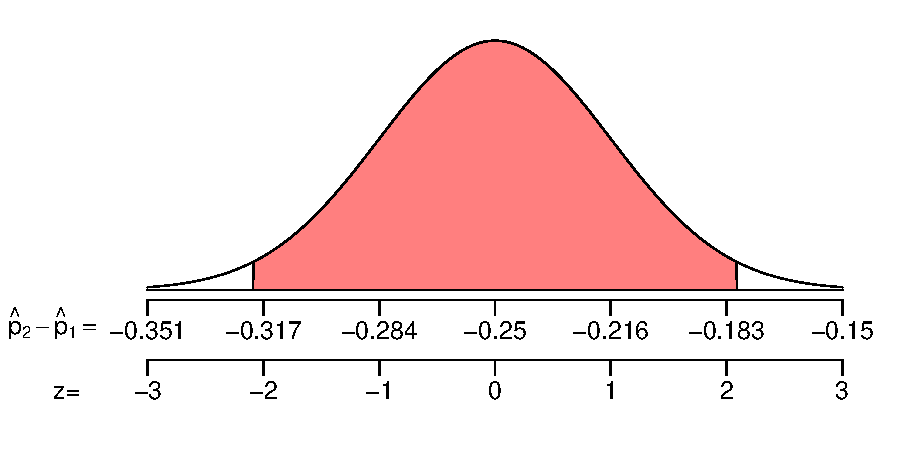
\includegraphics{diff_sampling_central_area-1.pdf} ~

Use a z table. \[
\begin{aligned}
\text{Pr}\left(0.29 < \hat{P}_2 - \hat{P}_1 < 0.316\right) &= \text{Pr}(|Z|<0.21) \\
&= 2\cdot\Phi(0.21)-1 \\
&= 0.1664
\end{aligned}
\]

Thus, we conclude that there is a 16.64\% chance that
\(\hat{P}_2-\hat{P}_1\) is between 0.29 and 0.316.
\end{solution}

